\begin{figure*}[h!]
    \centering
    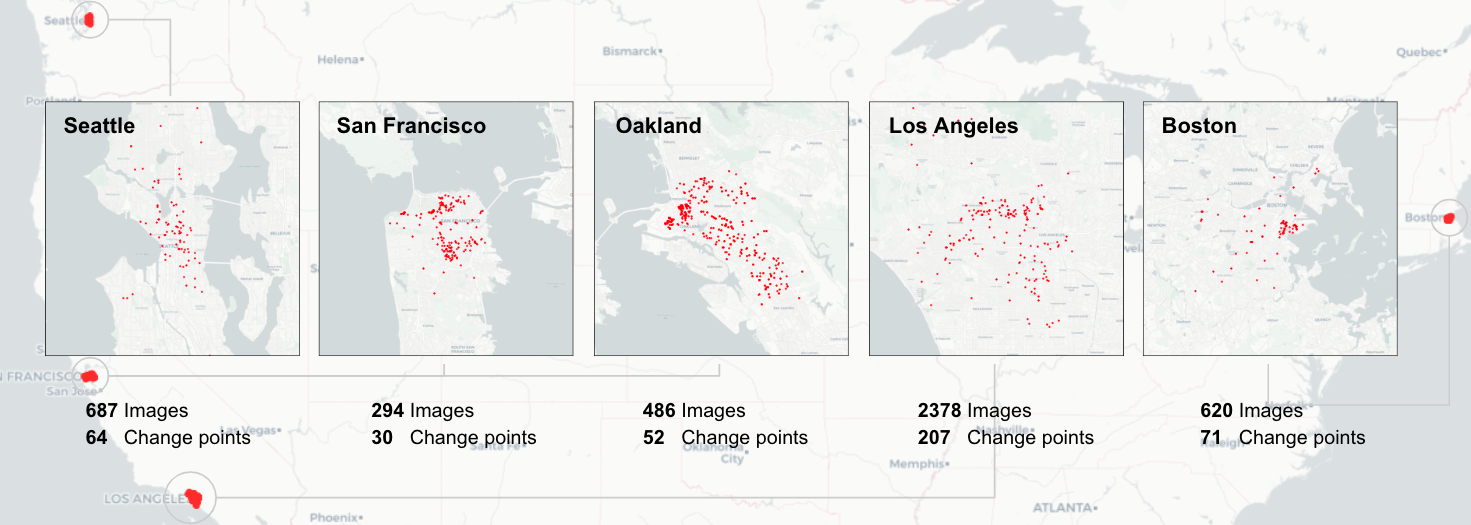
\includegraphics[width=0.98\linewidth]{figure/data_geo.png}
    \caption{Geo-spatial distribution of our street view time series dataset across 5 different cities in the US. Locations are selected based on open-access building footprint data, and historical Google Street View imagery from these coordinates is comprehensively downloaded and labeled with urban change points.}
    \label{fig:data_geo}
\end{figure*}

% \begin{figure*}[h!]
%     \centering
%     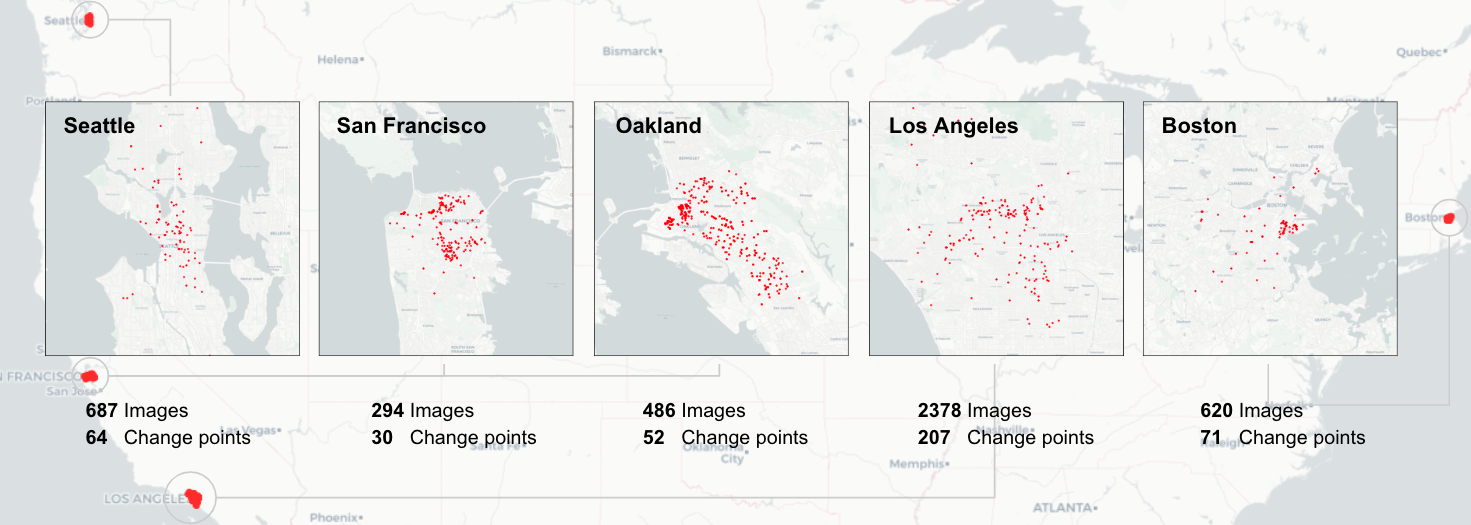
\includegraphics[width=0.98\linewidth]{figure/data_geo.png}
%     \caption{Geo-spatial distribution of our street view time series dataset. We sample street view time series data across 5 different cities in the US. Each location is determined through open-access building footprint data, and we download all the historical Google Street View that recorded there.}
%     \label{fig:data_geo}
% \end{figure*}